\documentclass[8pt]{beamer}

\usepackage[utf8]{inputenc}
\usepackage{default}
\usepackage{hyperref}
\usepackage{textpos}
\usepackage{color}
\usetheme{Copenhagen}

\title{Cybercom Machinebook}
\subtitle{Social Collaboration between People and Machines based on Conversational Paradigm, Machine Learning and Industrial Internet of Things}
\author{Tero Keski-Valkama}
\institute{
\includegraphics[height=1.4cm]{CybercomG_logo_Classic_RGB.png}}

\date{2016-08-16}
%\logo{
\includegraphics[height=1.2cm]{cybercom-blue.png}\vspace{195pt}}

\addtobeamertemplate{frametitle}{}{%
%\begin{textblock*}{100mm}(10.48cm,-0.8cm)
%
\includegraphics[height=1.2cm]{cybercom-blue.png}
%\begin{textblock*}{100mm}(10.48cm,-1.2cm)
%
\includegraphics[height=1.2cm]{cybercom-blue.png}
\begin{textblock*}{100mm}(10.95cm,-0.8cm)

\includegraphics[height=0.8cm]{cybercom-blue.png}
\end{textblock*}}

\begin{document}

\frame{\titlepage}

\begin{frame}
\frametitle{Machinebook at a Glance}
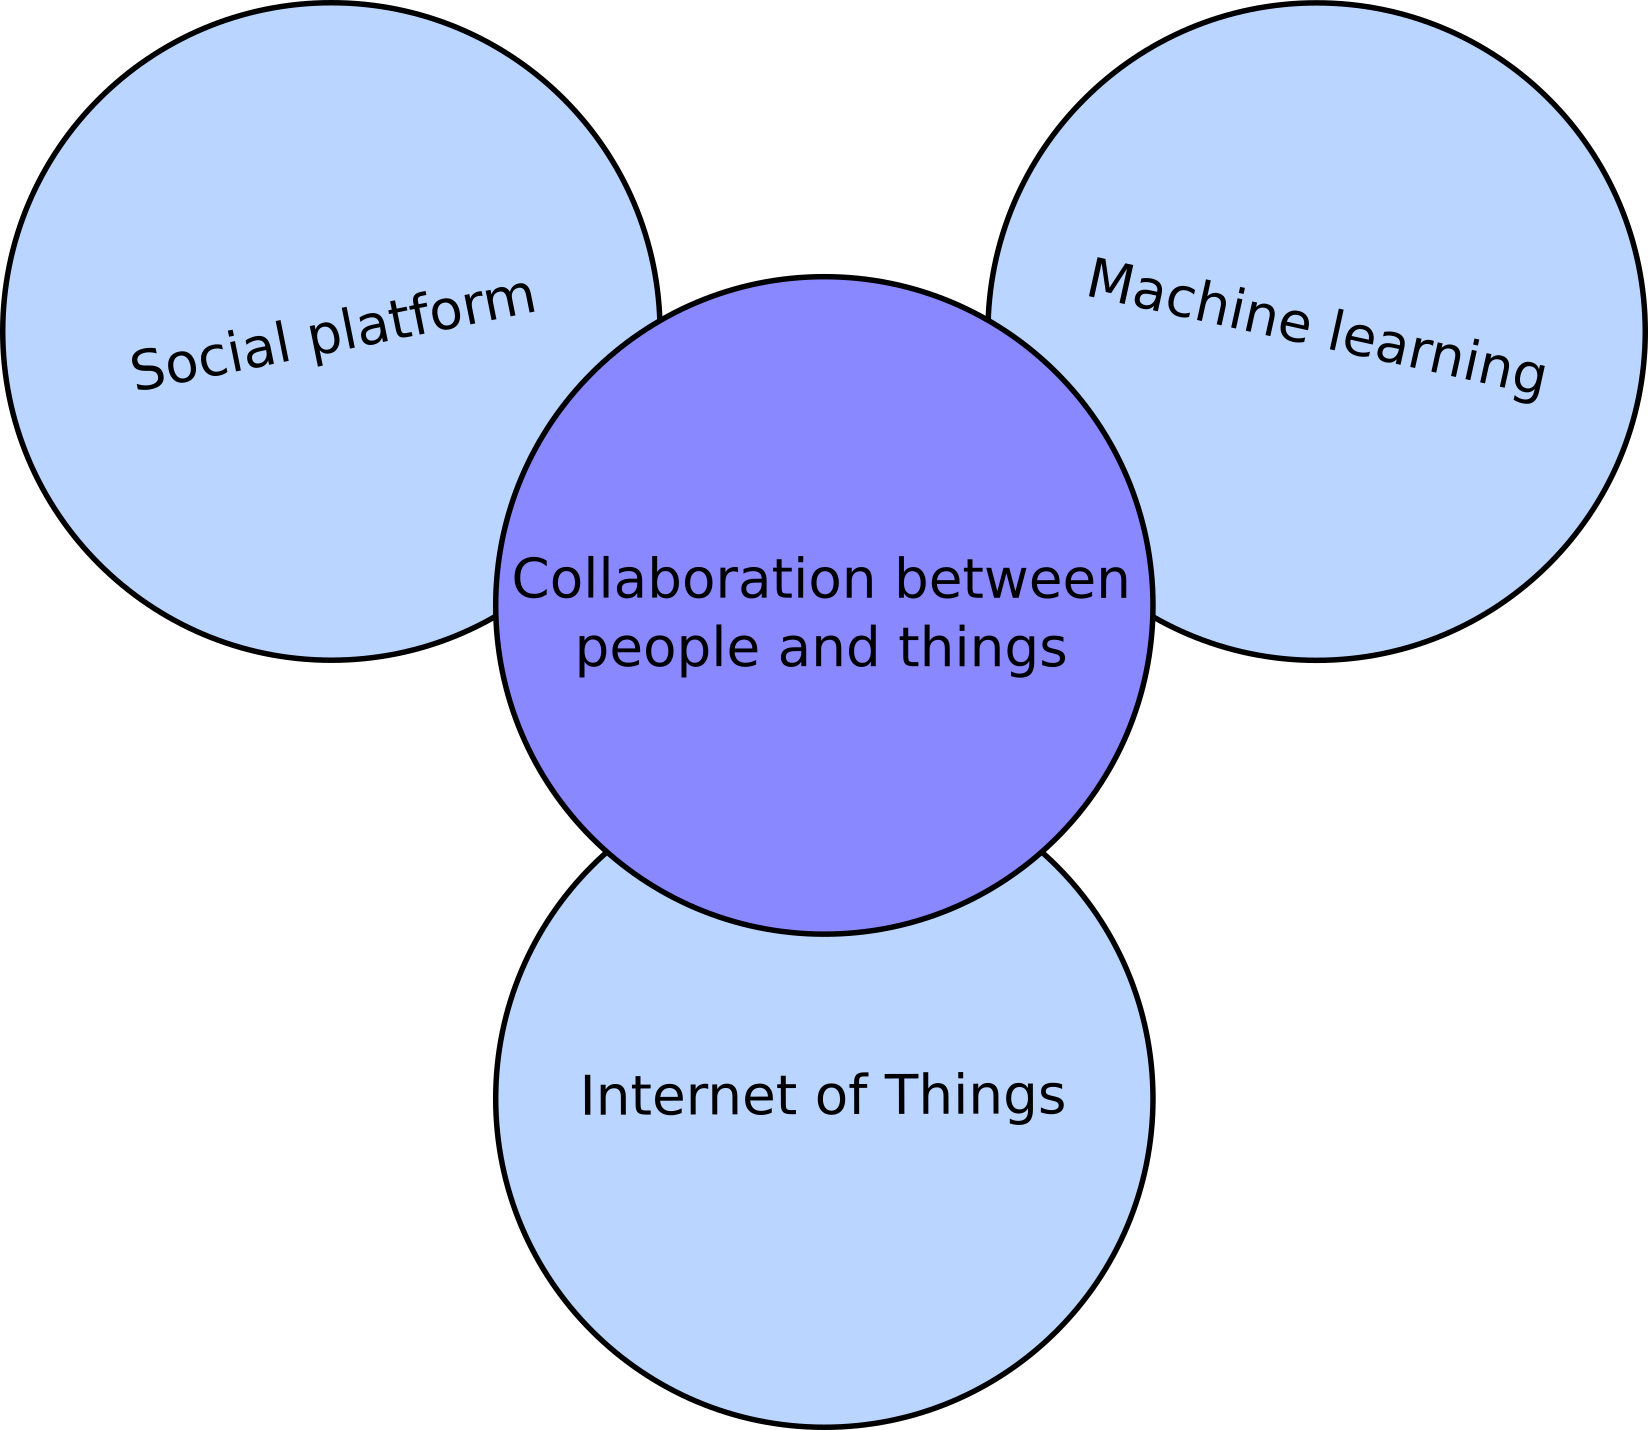
\includegraphics[width=0.9\textwidth]{./machinebook_concept.png}
\end{frame}

\begin{frame}
\frametitle{Machinebook}
\begin{itemize}
 \item \textbf{Machinebook is a concept which projects intelligent IoT machines onto a social collaboration platform as avatars.}
 \item Conversational interface is an emerging paradigm in consumer products and services, not yet taken into use in the industrial context.
 \item Social platform enables deployment of effective machine intelligence technologies. Mining conversations has standard tools, and can be more convenient for
       many use cases than special queries to structured databases. Conversational capabilities can be incrementally developed and deployed without designing
       new user interfaces each time. Integrating intelligent capabilities behind a conversational avatar can be more natural in some cases than creating dashboards.
 \item Invisible, separate IoT logs become visible, shared \textbf{stories} and people and machines are on the same page on what is happening.
       Social interactions bring silent knowledge and experience explicit.
\end{itemize}
\centering{
 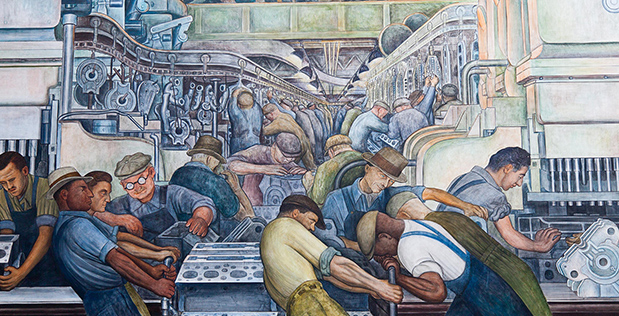
\includegraphics[width=0.5\textwidth]{./tehdas.jpg}
}
\end{frame}
      
\begin{frame}
\frametitle{Machinebook}
\begin{itemize}
 \item A social avatar is like \textbf{a working dog}, not a hammer. Social avatars form \textbf{a team}, not a massive bag of separate tools.
       The social avatars are taught like colleagues, instead of programming them as asocial automation systems.
 \item Avatars represent the machine provider, the site management and the machine itself. They provide a channel for user guides, maintenance assistance, after market sales,
       task assistance, and even motivation and customer company values.
 \item Marketplace for components allows progressive development and deployment of incremental intelligent functionality.
\end{itemize}
\centering{
 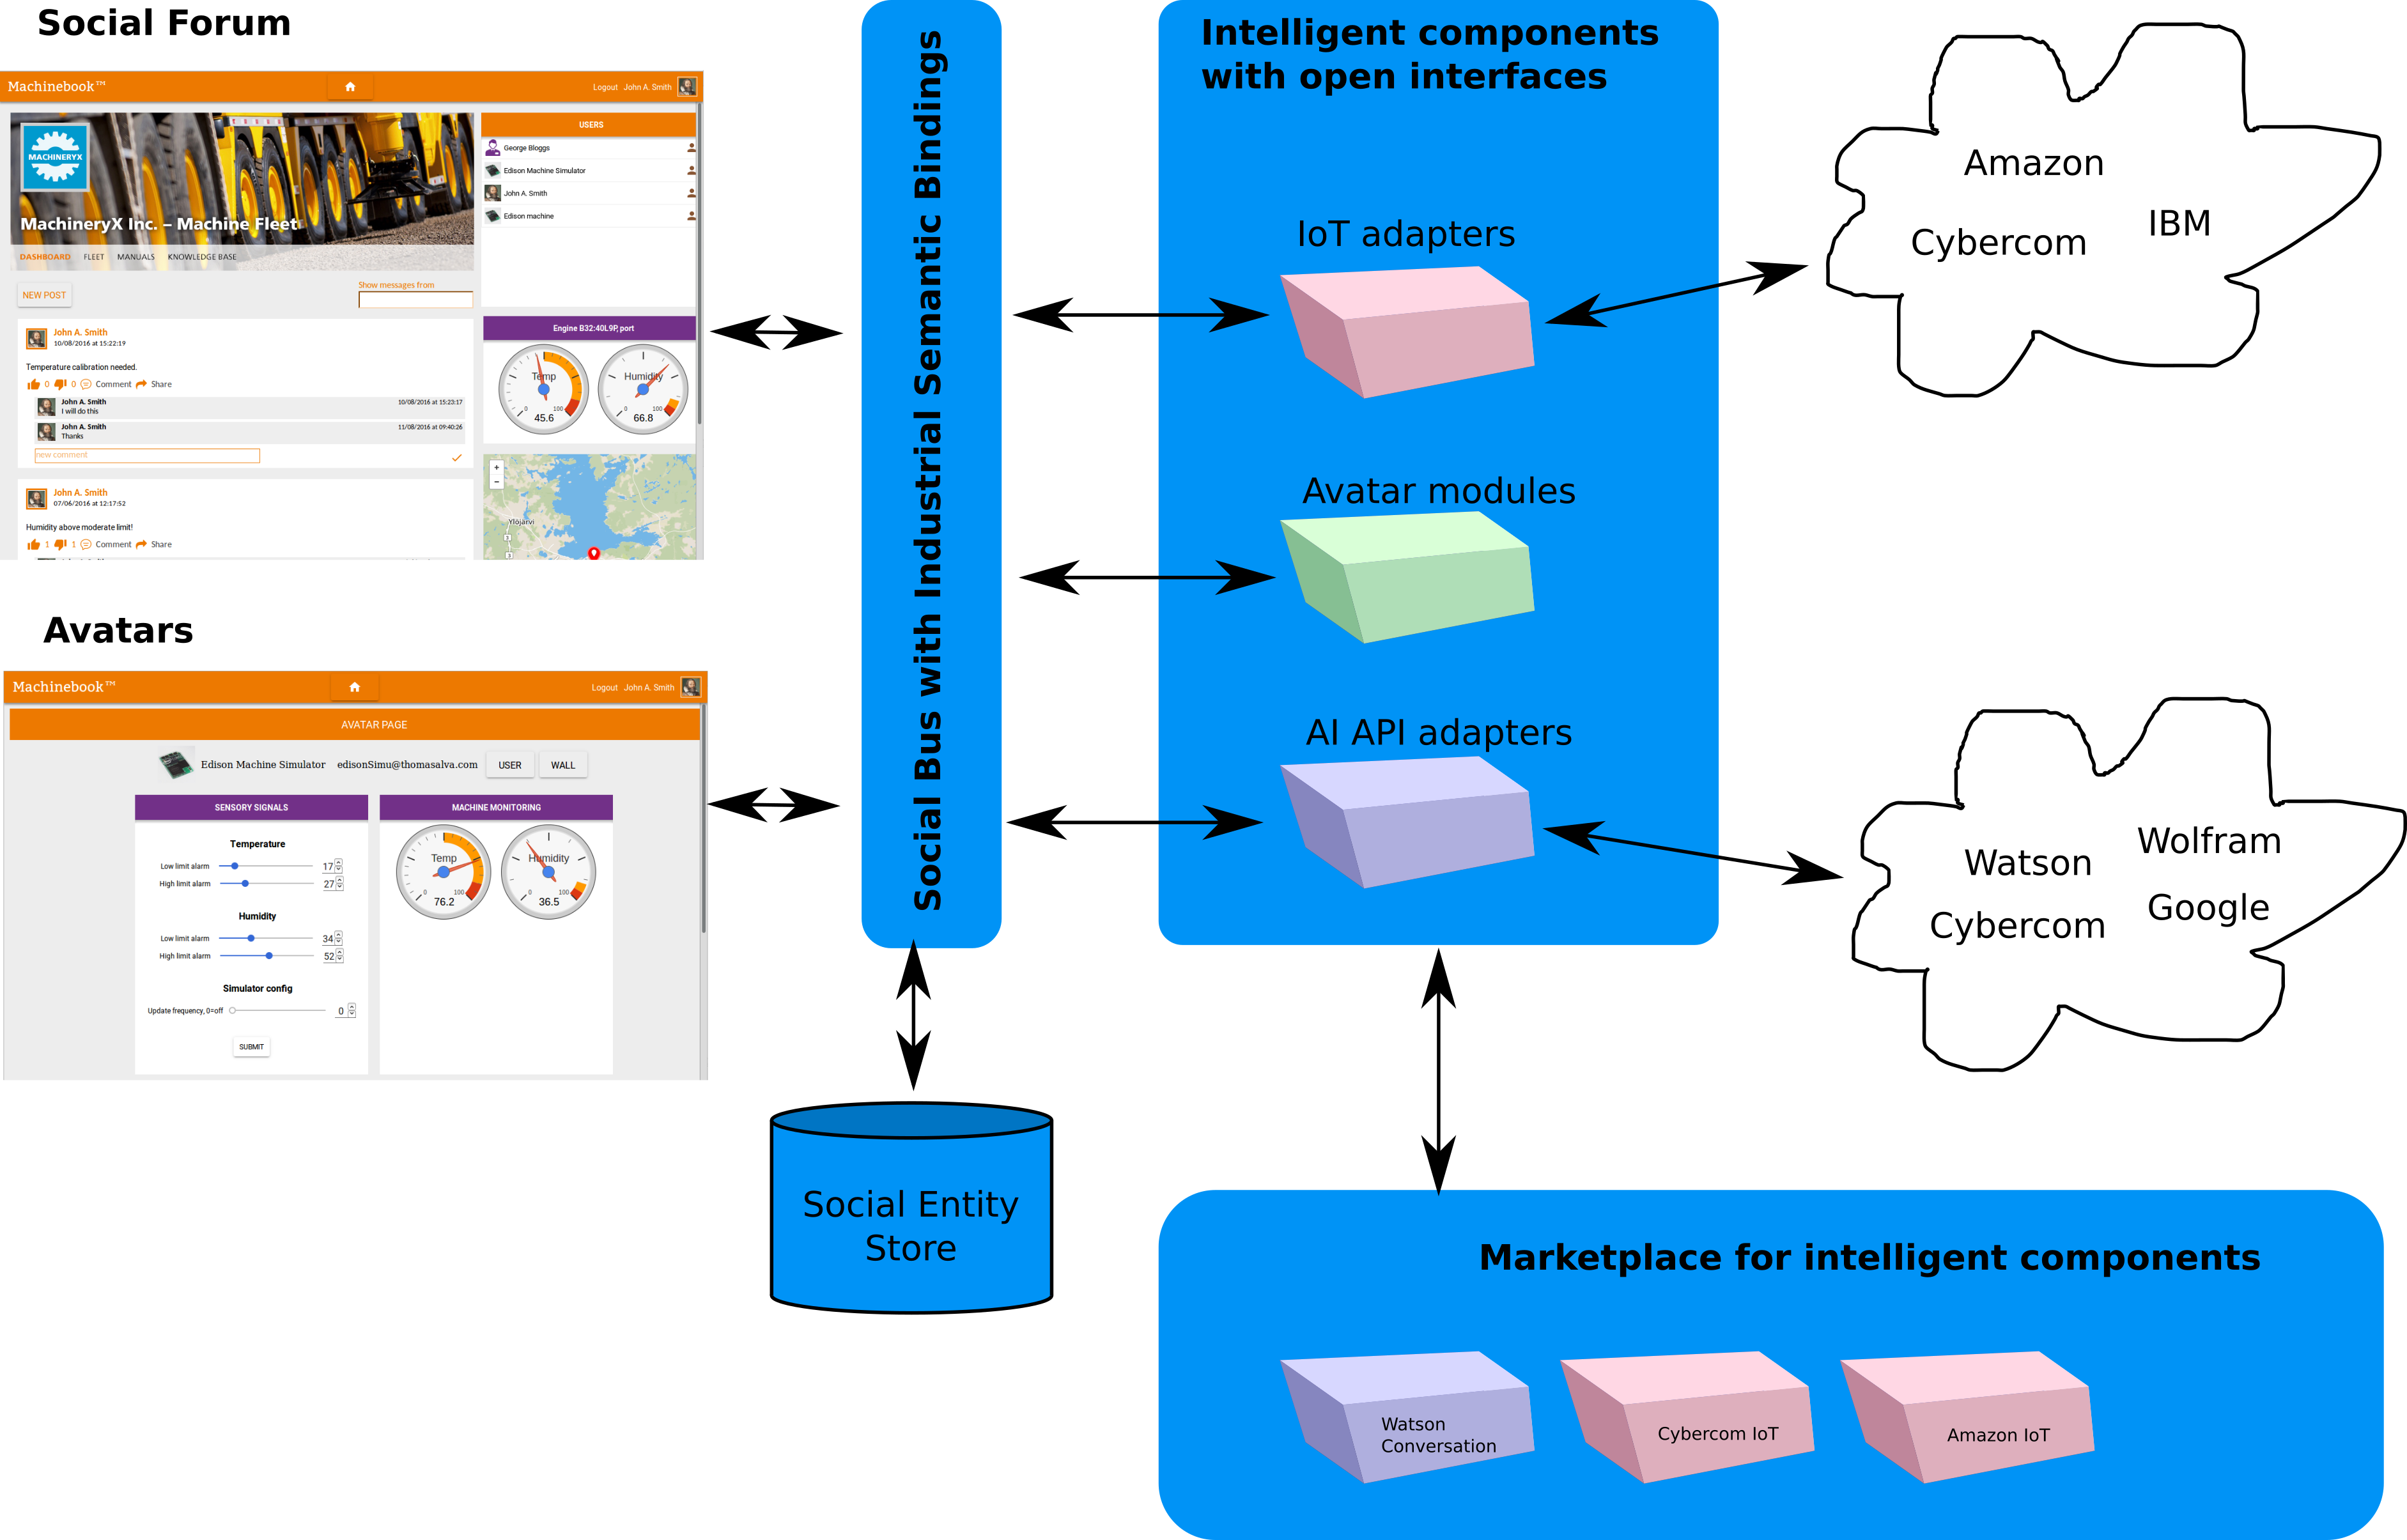
\includegraphics[width=0.6\textwidth]{./mb_architecture.png}
}

\end{frame}

\begin{frame}
\frametitle{Links}
\begin{itemize}
 \item Machinebook has generated intense interest in media and in business circles both in Finland and internationally.
 \item \textcolor{blue}{\href{http://www.aamulehti.fi/kotimaa/hervannassa-on-kehitetty-koneille-omaa-facebookia/}{Tampereella on kehitetty koneille omaa "Facebookia" – Aamulehti}}
 \item \textcolor{blue}{\href{http://www.kauppalehti.fi/uutiset/cybercom-loi-ihmisten-ja-koneiden-somen/nrWndBBV}{Cybercom loi ihmisten ja koneiden somen – Kauppalehti}}
 \item \textcolor{blue}{\href{http://www.redeye.se/aktieguiden/nyheter/it-machinebook-blir-maskinernas-sociala-natverk}{IT: ``MACHINEBOOK'' BLIR MASKINERNAS SOCIALA NÄTVERK – RedEye.se}}
 \item \textcolor{blue}{\href{http://www.cybercom.com/About-Cybercom/Blogs/the-connected-world/machinebook/}{The latest blog post about Machinebook}}
\end{itemize}
\centering{
 \includegraphics[width=0.27\textwidth]{./tehdaskone.png}
}
\centering{
 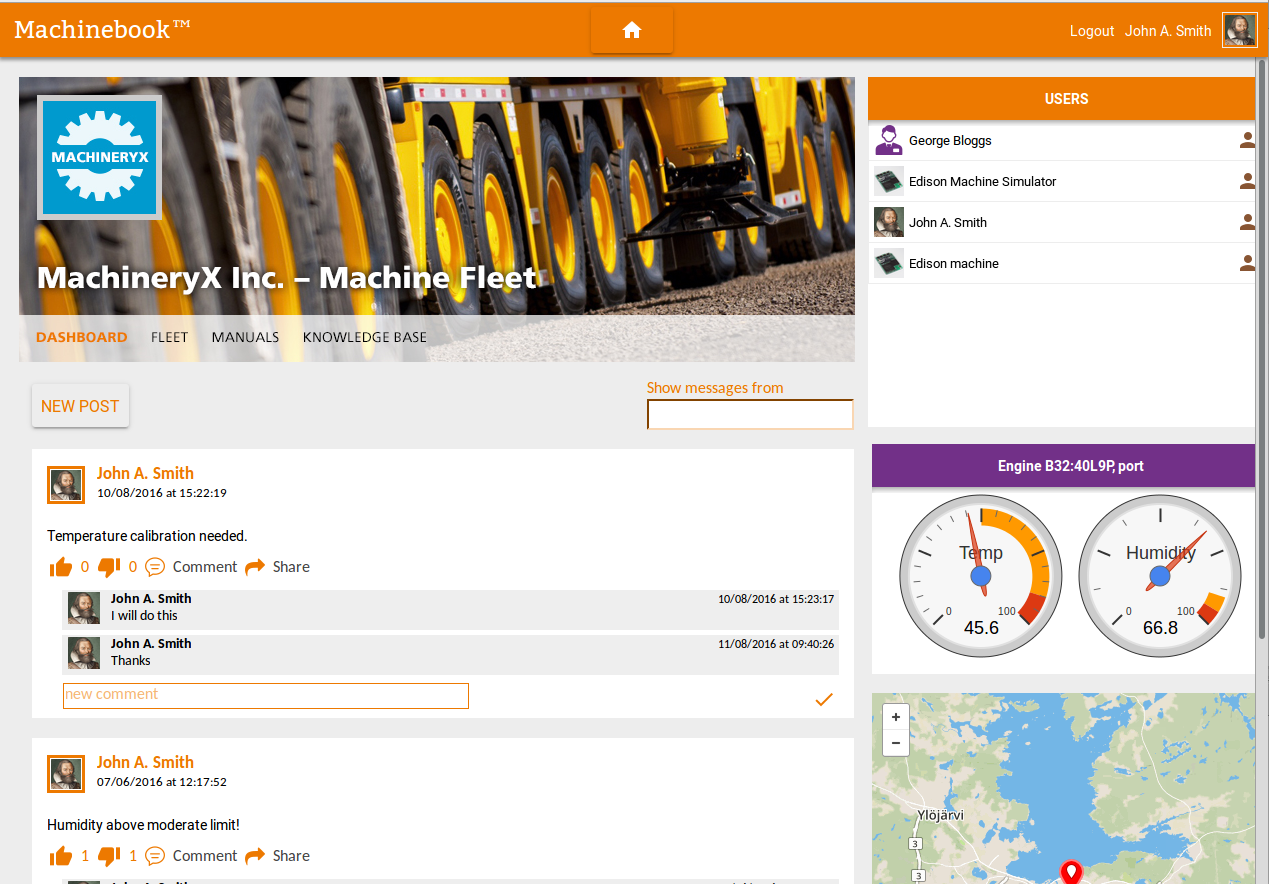
\includegraphics[width=0.4\textwidth]{./wall.png}
 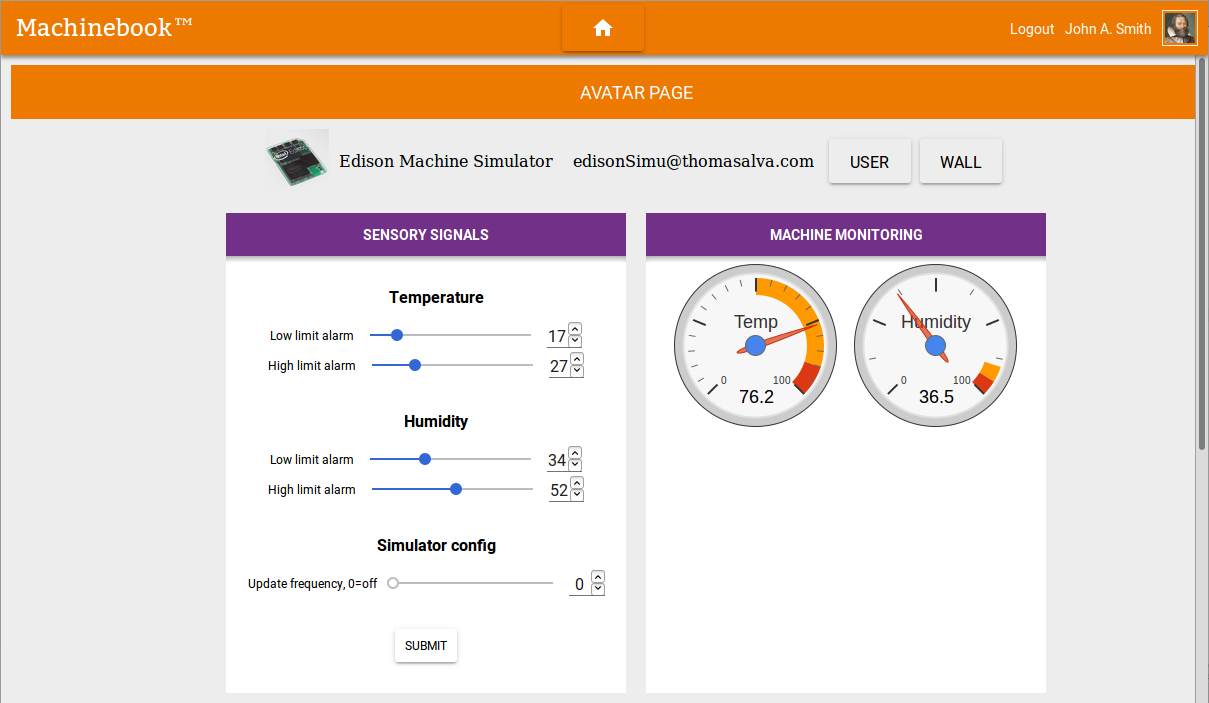
\includegraphics[width=0.478\textwidth]{./avatar.png}
}
\end{frame}
\end{document}
